\documentclass{article}

\usepackage{amsmath}
\usepackage{amsthm}
\usepackage{amssymb}
\usepackage{mathtools}

\usepackage{tikz}
\usetikzlibrary{calc, intersections}


\title{Analysuppgift 5 - Area under kurvor}
\author{Emma Bastås}
\date{November 6, 2022}

\begin{document}

\maketitle

\noindent Uppgiften är att beräkna arean av de område som begränsas av kurvorna $y = f(x)$ och $y = g(x)$ där:

\begin{gather*}
  f(x) = x^{2} \quad\text{och}\quad g(x) = 2 - x\text{.}
\end{gather*}
\\
\\
Utan att göra någon mer detaljerad analys av kurvornas utseende så kan vi ändå säga att grafen till dessa två kurvor kring origo ser ut ungefär såhär:

\begin{center}
  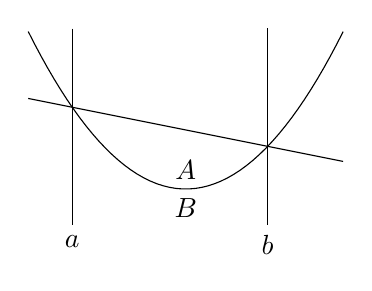
\begin{tikzpicture}
%\draw[name path=line,smooth] (0,5)--(1.5,5);
%\draw[name path=curve,smooth] (1.5,6) to[out=270,in=90] (0,3);
%\draw[name intersections={of=line and curve}] (intersection-1) circle[radius=0.1];
    \draw [name path=parabola, domain=-2:2, samples=50] plot (\x, 0.5*\x*\x) node[midway, below] {$B$};
    \draw [name path=line, domain=-2:2, samples=50] plot (\x, 0.75 - 0.20*\x) node[midway, above] {$A$};
    \draw[name intersections={of=line and parabola}] (intersection-1) ++(0, 1) -- +(0,-2.5) node[pos=1, below] {$a$};
    \draw[name intersections={of=line and parabola}] (intersection-2) ++(0, 1.5) -- +(0,-2.5) node[pos=1, below] {$b$};
  \end{tikzpicture}
\end{center}

\noindent Vi har här gjort två antaganden:

\begin{enumerate}
        \item linjen $y = g(x)$ skär kurvan $y = f(x)$ i två skilda punkter $x = a$ och $x = b$. Detta kommer vi senare att verifiera.
        \item Ingen av kurvorna går under $x$-axeln i intervallet $[a,b]$. Det är uppenbart att $y = f(x)$ aldrig går under $x$-axeln, om det första antagandet gäller så kommer heller aldrig linjen $y = g(x)$ att skära $x$-axeln i intervallet.
\end{enumerate}

\noindent Det som vi ska beräkna är arean av området $A$. Arean under $y = f(x)$ i området $[a, b]$ ges av $\int_{a}^{b} f(x) \,\mathrm{d}x = B$. Arean under $y = g(x)$ i området $[a, b]$ ges av $\int_{a}^{b} g(x) \,\mathrm{d}x = A + B$. Vi får då ett uttryck för arean $A$:

\begin{gather}
  A = (A + B) - B = \int_{a}^{b} g(x) \,\mathrm{d}x - \int_{a}^{b} f(x) \,\mathrm{d}x\text{.} \label{1}
\end{gather}

\noindent Både $f(x)$ och $g(x)$ är kontinuerliga för alla reella värden på $x$. Om $F(x)$ och $G(x)$ är primitiva funktion till $f(x)$ respektive $g(x)$ ger analysens huvudsats att:

\begin{align}
  \text{(\ref{1})} &= (G(b) - G(a)) - (F(b) - F(a)) \notag\\
  &= G(b) - G(a) - F(b) + F(a)\text{.} \label{2}
\end{align}

\noindent Det som återstår nu är att finna primitiva funktioner till $f(x)$ och $g(x)$ samt skärningspunkterna $a$ och $b$.
\\
\\
\noindent Skärningspunkterna $a$ och $b$ är lösningarna till andragradsekvationen $f(x) = g(x)$, de två lösningarna är $x = -2$ och $x = 1$, d.v.s $a = -2$ och $b = 1$. Nu har vi även verifierat att antagandena som vi gjorde om kurvorna tidigare gäller.
\\
\\
\noindent Att finna primitiva funktioner görs med integreringsregler för polynom. Vi finner att $F(x) =\tfrac{1}{3}x^{3} + C$ och $G(x) = 2x - \tfrac{1}{2}x^{2} + D$ där $C$ och $D$ är två okända konstanter.
\\
\\
\noindent Det som återstår nu är att beräkna värdet på (\ref{2}):

\begin{gather*}
  G(1) - G(-2) - F(1) + F(-2) = \frac{9}{2}\text{.}
\end{gather*}

\noindent Vi har alltså visat att $A = \frac{9}{2}$ vilket är vad som söktes.
\\
\\

\centering{$\qed$}

\end{document}
